\subsection{Triple Integrals}

\content{
\begin{definition} The triple integral of $f$ over the box 
$B = [a,b]\times [c,d]\times[e,f]$ is given by 
$$\iiint_B f(x,y,z)\,dV =\lim_{i,j,k\rightarrow}\sum_{i=1}^\ell\sum_{j=1}^m
\sum_{k=1}^n f(x_{ijk}^*,y_{ijk}^*,z_{ijk}^*)\Delta V$$
\end{definition}
}{% presentation
}{% nopresentation
}{% comments
}

\content{
\begin{theorem} If $f$ is continuous on the box $B$, then 
$$ \iiint_B f(x,y,z)\, dV = \int_a^b\int_c^d\int_e^f 
f(x,y,z) \,dz dy dx. $$
\end{theorem}
}{% presentation
}{% nopresentation
}{% comments
Mention that there are five other orders which we can choose here, all of which
are the same. 
}

\content{
\begin{example} Evaluate the integral $\iiint_B xyz^2\,dV$ where 
$B = [0,1]\times[-1,2]\times[0,3]. $
\end{example}
}{% presentation
\vspace{3in}
}{% nopresentation
\vspace{2in}
}{% comments
Answer is $\frac{27}{4}$.
}

\content{
\begin{example} Evaluate the integral $\iiint_E z\, dV$, where $E$ is the solid
in the first octant bounded by the surface $z=12xy$ and the planes $y=x$, and
$x=1$.
\end{example}
}{% presentation
\vspace{4in}
}{% nopresentation
\vspace{2in}
\newpage
}{% comments
mention that just as in the case of double integrals, we can define the integral
of more complicated regions like the one in this example. 
}

\content{
\begin{example} Evaluate the integral $\iiint_E \sqrt{x^2+z^2}\,dV$ where 
$E$ is the region bounded by the paraboloid $y=x^2+z^2$ and the plane $y=4$.
\end{example}
}{% presentation
\vspace{4in}
}{% nopresentation
\vspace{3in}
}{% comments
        Answer is $8\pi$.
}

\content{
\begin{example} Use a triple integral to find the volume of the tetrahedron $T$
bounded by the planes $x+2y+z=2$, $x=2y$, $y=0$ and $z=0$.
\end{example}
}{% presentation
}{% nopresentation
\vspace{2in}

}{% comments
}

\newpage
\subsection{More Practice with Triple Integrals}

\content{
        \begin{example} Set up the triple integral $\iiint_E x \, dV$ where E is
        the solid shown below:\\
        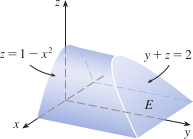
\includegraphics{img/24-1.png}
        \end{example}
}{% presentation
}{% nopresentation
}{% comments
}

\content{
        \begin{example}
        Set up the triple integral $\iiint_E xy\, dV$ where E is the solid shown
        below:\\
        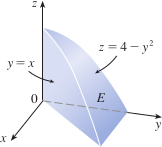
\includegraphics{img/24-2.png}
        \end{example}
}{% presentation
}{% nopresentation
}{% comments
}

\content{
        \begin{example}
        Set up the triple integral $\iiint_E 2\, dV$ where E is the solid shown
        below:\\
        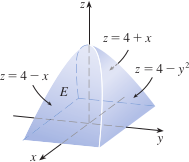
\includegraphics{img/24-3.png}
        \end{example}
}{% presentation
}{% nopresentation
}{% comments
}

\content{
        \begin{example}
        Set up the triple integral $\iiint_E 2\, dV$ where E is the solid
        bounded by the surfaces $z = x^2 - 1$, $z = 1-x^2$, $y=0$ and
        $y=2$.
        \end{example}
}{% presentation
        \vspace{0.5in}
}{% nopresentation
}{% comments
}

\content{
        \begin{example}
                Set up a triple integral to find the volume of the solid bounded
                by the coordinate planes and the plane $2x+y+z=4$.
        \end{example}
}{% presentation
        \vspace{0.5in}
}{% nopresentation
}{% comments
}
